\subsubsection{Preparación de clase por parte de un profesor}

{\textbf {Resumen:}}
El nuevo director de UTP le dice al profesor de Historia de la existencia de una nueva App de Museos, el director quiere que el profesor haga uso de la aplicación en su clase. El profesor en su casa descarga la aplicación, imprime el código del museo que quiere mostrar en clases y empieza a buscar piezas, el profesor se da cuenta de que la app tiene logros, así que busca la manera de utilizar esos logros como décimas para la siguiente prueba del análisis de un museo histórico, en cuanto un alumno consiga un logro, se le asignará una décima. Ya en la clase el profesor empieza a mostrar la aplicación y enseña cómo obtener una pieza y muestra el tutorial completo de la manipulación de la pieza en 3d para ver los detalles de los modelos.


{\textbf {Actores:}}
Profesor, Director.

{\textbf {Propósito:}}
Demostrar el uso de la aplicación como herramienta de apoyo educativa dentro y fuera del aula.

{\textbf {Referencias cruzadas:}}
XXXX

\paragraph{Caso de Uso Esencial}

\begin{longtable}{|p{5cm}|p{8cm}|}
\hline 
Acción actores & Respuesta del sistema \\ 
\hline 
El profesor abre la aplicación y presiona sobre el botón de piezas. & El sistema despliega un menú con todas las piezas, con toda la información de las que han sido descubiertas y con la mínima de las que no. \\ 
\hline
El profesor elige una de las piezas que son de interés para su clase y la selecciona. & Se despliega una escena con la pieza seleccionada , muestra un panel con el tutorial para poder manipular esta pieza y poder verla en todo los ángulos y posiciones posibles. \\ 
\hline 
El profesor ocupa la aplicación y va mostrando los detalles de las piezas a los alumnos. & El tutorial es achicado y desplazado a un costado para que sea siempres visible pero no obstaculice el manejo de la pieza. \\ 
\hline 
\end{longtable}

\paragraph{Diagrama de Caso de Uso}

\begin{figure}[H]
\centerline{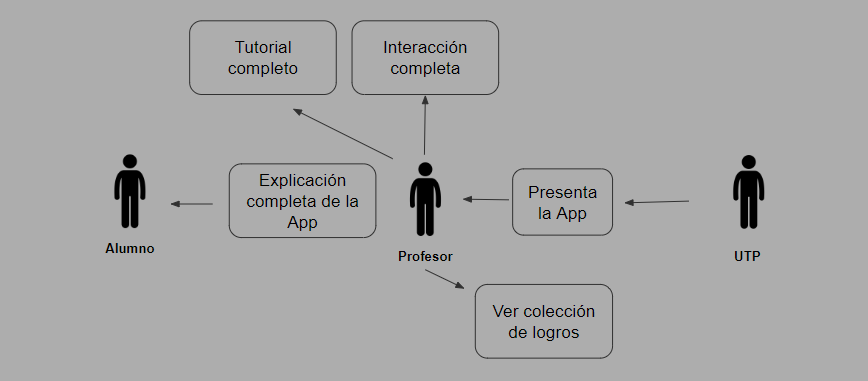
\includegraphics[width=15cm]{imgs/CasoUso_8.PNG}}
\caption{Caso-1}
\label{fig}
\end{figure}

\paragraph{Modelo Conceptual}

\begin{figure}[H]
\centerline{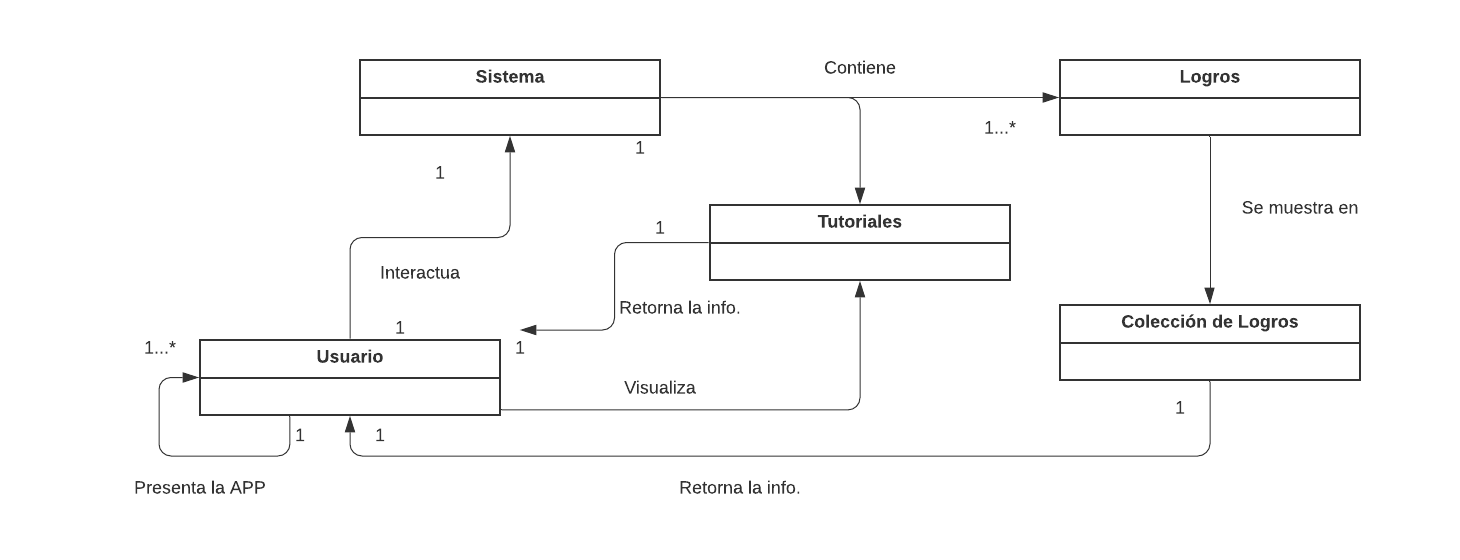
\includegraphics[width=15cm]{imgs/ModeloConceptualCaso_8_3.png}}
\caption{Caso-1}
\label{fig}
\end{figure}

\paragraph{Diagrama de Secuencia o Colaboración}

\begin{figure}[H]
\centerline{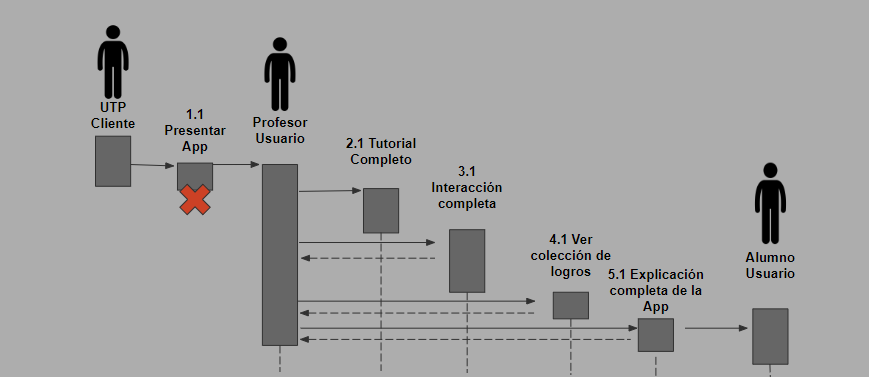
\includegraphics[width=15cm]{imgs/CasoUso_8_2.PNG}}
\caption{Caso-1}
\label{fig}
\end{figure}

\paragraph{Priorización}
{\textbf {Tipo:}}
Esencial.